\documentclass[12pt,a4paper]{article}
\usepackage{graphicx}
\usepackage{amsmath}
\usepackage{amssymb}
\usepackage{listings}
\usepackage{geometry}
\usepackage{multicol}
\geometry{margin=1in}
\begin{document}
\noindent

\begin{minipage}{0.6\textwidth}

\includegraphics[width=0.75\textwidth]{IIITB-COMET-Logo.png}
\end{minipage}
\begin{minipage}{0.38\textwidth}
\begin{center}
\textbf{DARSI VAMSI}
\newline
\textbf{COMET FWC 071}
\end{center}
\end{minipage}
\newline
\newline
\begin{center}
    {\LARGE\textbf{Implementation of the Boolean Function}}\\[0.3cm]
    {\LARGE\textbf{$Y=AB+CD$ Using Raspberry Pi Pico 2 W with 7447 IC }}
    \\
    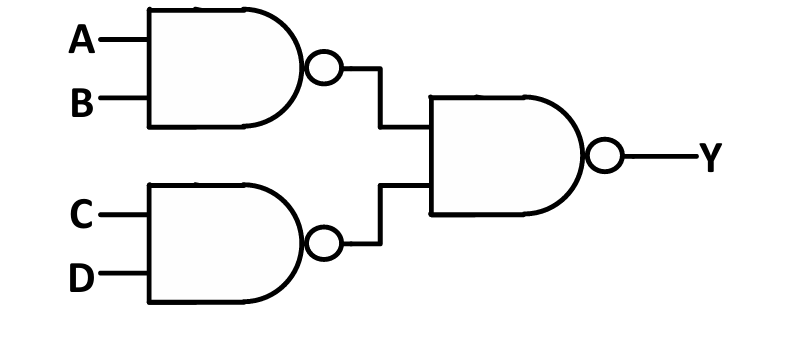
\includegraphics[width=0.75\textwidth]{figure.png}
\end{center}

\section{Problem Analysis}

The given logic circuit consists of three NAND gates.

The output of the first NAND gate is

$$
X_1=(AB)'
$$

The output of the second NAND gate is

$$
X_2=(CD)'
$$

The final output is

$$
Y=(X_1X_2)'
$$

Substituting the values of $X_1$ and $X_2$,

$$
Y=((AB)'(CD)')'
$$

Applying De Morgan's theorem,

$$
Y=((AB)')'+((CD)')'
$$

Therefore,

$$
\boxed{Y=AB+CD}
$$

The output becomes logic '1' whenever:

\begin{itemize}
    \item $A=1$ and $B=1$, or
    \item $C=1$ and $D=1$.
\end{itemize}

Otherwise, the output remains logic '0'.
\section{Hardware Requirements}

\renewcommand{\arraystretch}{1.3}

\begin{center}
\begin{tabular}{|c|p{9cm}|}
\hline
\textbf{S.No.} & \textbf{Component} \\
\hline
1 & Raspberry Pi Pico 2 W Development Board \\
\hline
2 & IC 7447 BCD-to-7-Segment Decoder \\
\hline
3 & Common Anode Seven-Segment Display \\
\hline
4 & Breadboard \\
\hline
5 & USB Type-C Cable \\
\hline
6 & Connecting Wires \\
\hline
7 & 220 $\Omega$ Resistors (Optional for Segment Protection) \\
\hline
8 & Personal Computer or Laptop \\
\hline
\end{tabular}
\end{center}
\section{Pin Connections}

\subsection{Raspberry Pi Pico 2W to 7447 IC Connections}

\begin{table}[h!]
\centering
\renewcommand{\arraystretch}{1.3}
\begin{tabular}{|c|c|c|}
\hline
\textbf{Raspberry Pi Pico 2W Pin} & \textbf{7447 Input Pin} & \textbf{Signal Name} \\
\hline
GP8  & A & Input A (LSB) \\
\hline
GP9  & B & Input B \\
\hline
GP10 & C & Input C \\
\hline
GP11 & D & Input D (MSB) \\
\hline
GND  & GND & Ground \\
\hline
5V   & VCC & Power Supply \\
\hline
\end{tabular}
\caption{Connections between Raspberry Pi Pico 2W and 7447 IC}
\end{table}

\subsection{7447 IC to 7-Segment Display Connections}

\begin{table}[h!]
\centering
\renewcommand{\arraystretch}{1.3}
\begin{tabular}{|c|c|c|}
\hline
\textbf{7447 Output Pin} & \textbf{7-Segment Pin} & \textbf{Segment} \\
\hline
a & a & Segment A \\
\hline
b & b & Segment B \\
\hline
c & c & Segment C \\
\hline
d & d & Segment D \\
\hline
e & e & Segment E \\
\hline
f & f & Segment F \\
\hline
g & g & Segment G \\
\hline
VCC & Common Anode & Power Supply \\
\hline
GND & GND (via IC) & Ground Reference \\
\hline
\end{tabular}
\caption{Connections between 7447 IC and 7-Segment Display}
\end{table}
\section{Hardware Setup and Accessing Raspberry Pi Pico 2 W Using Arduino IDE}

The Raspberry Pi Pico 2 W is programmed using the Arduino IDE by installing the necessary board support packages and configuring the development environment. The detailed procedure is as follows.



\subsection{Installing Arduino IDE}

\begin{enumerate}
    \item Download and install the latest version of Arduino IDE from the official Arduino website.
    \item Open the Arduino IDE after installation.
\end{enumerate}

\subsection{Installing Raspberry Pi Pico 2 W Board Package}

\begin{enumerate}
    \item Open Arduino IDE.
    \item Navigate to
    \[
    \text{File} \rightarrow \text{Preferences}
    \]
    
    \item In the ``Additional Boards Manager URLs'' field, add the following URL:
    
\begin{verbatim}
https://github.com/earlephilhower/arduino-pico/releases/download/global/package_rp2040_index.json
\end{verbatim}

    \item Click ``OK''.
    
    \item Navigate to
    \[
    \text{Tools} \rightarrow \text{Board} \rightarrow \text{Boards Manager}
    \]

    \item Search for ``Raspberry Pi Pico/RP2040''.

    \item Install the package developed by Earle F. Philhower.
\end{enumerate}

\subsection{Connecting the Raspberry Pi Pico 2 W}

\begin{enumerate}
    \item Connect the Raspberry Pi Pico 2 W to the computer using a USB Type-C cable.
    
    \item If the board is not detected automatically:
    \begin{enumerate}
        \item Press and hold the \textbf{BOOTSEL} button.
        \item Connect the USB cable while holding the button.
        \item Release the button after the board appears as a removable drive.
    \end{enumerate}
\end{enumerate}

\subsection{Selecting the Board and Port}

\begin{enumerate}
    \item Navigate to
    \[
    \text{Tools} \rightarrow \text{Board}
    \]

    \item Select
    \[
    \text{Raspberry Pi Pico 2 W}
    \]

    \item Navigate to
    \[
    \text{Tools} \rightarrow \text{Port}
    \]

    \item Select the corresponding COM port of the Raspberry Pi Pico 2 W.
\end{enumerate}

\subsection{Uploading the Program}

\begin{enumerate}
    \item Write or paste the Arduino program into the Arduino IDE.
    \item Click the \textbf{Verify} button to compile the code.
    \item Click the \textbf{Upload} button.
    \item Wait until the message

Done Uploading\\
appears in the output window.
\end{enumerate}


After successful uploading of the program, the Raspberry Pi Pico 2 W executes the Boolean expression

$$
Y = AB + CD
$$

for all possible input combinations and displays the output through the LED connected to GP1.
\section{Results Obtained in the Experiment}

The Boolean function implemented is:
$$
Y = (A \cdot B) + (C \cdot D)
$$

The output was observed for all possible input combinations. The results are categorized based on the output value.
\newpage\begin{multicols}{2}
\subsection{Combinations for Output $Y = 0$}
The below combinations provides the output as zero.\\
The observations are tabulated below.\\



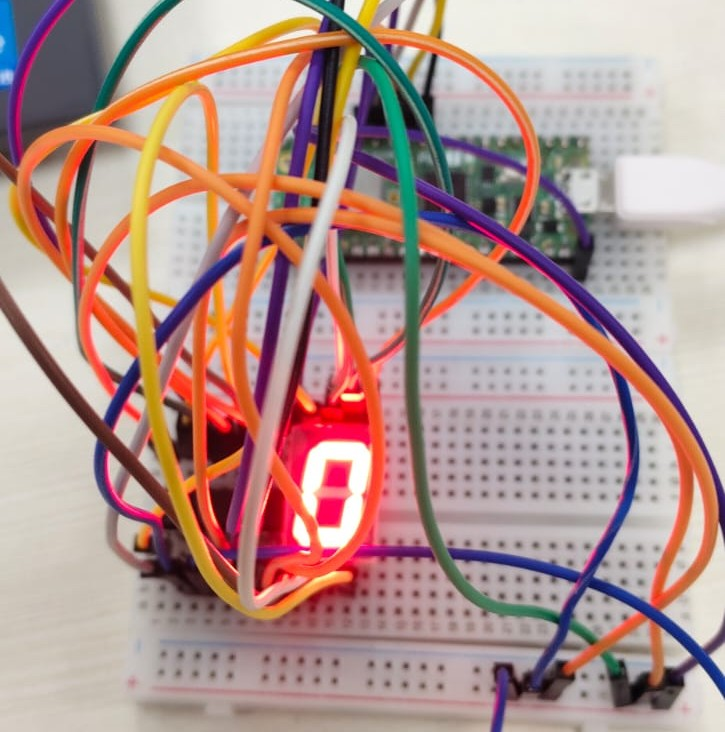
\includegraphics[width=0.3\textwidth,height=0.3\textheight]{output_as_1.jpeg}

\subsection{Combinations for Output $Y = 1$}

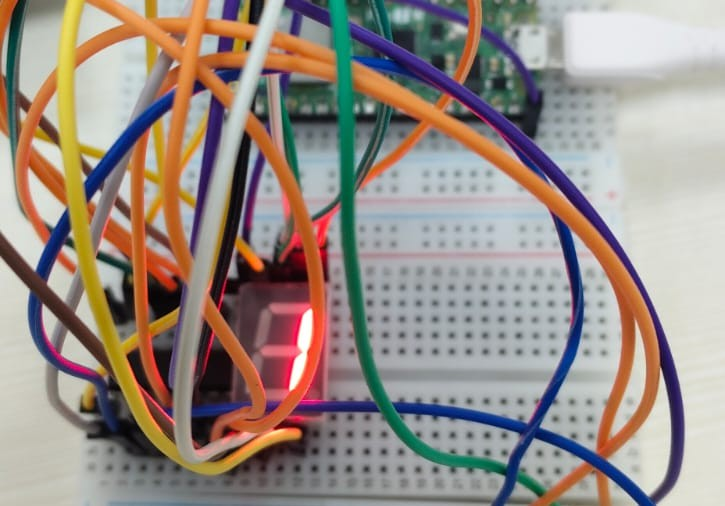
\includegraphics[width=0.3\textwidth,height=0.3\textheight]{output_as_one.jpeg}

\end{multicols}

\end{document}